\chapter{Appendix}
\section{Zeitaufwand}
Der gearbeitete Zeitaufwand für Shulker ist in folgenden Diagrammen ersichtlich:

\subsection{Zeitaufwand Alexander Heim}
\textbf{Zeitaufwand}
\begin{figure}[H]
    \begin{center}
        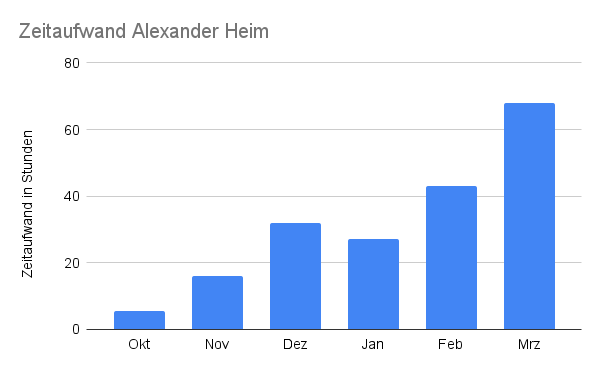
\includegraphics[width=.75\textwidth]{images/appendix/ZeitaufwandHeim.png}
        \caption{Arbeitsstunden von Alexander Heim verteilt auf die Monate}
    \end{center}
\end{figure}

\textbf{Verteilung der Arbeitszeit}
\begin{figure}[H]
    \begin{center}
        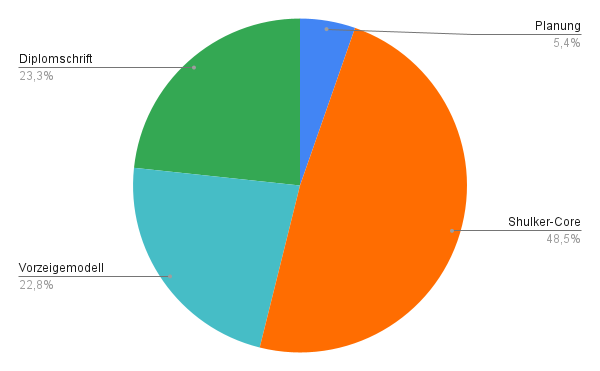
\includegraphics[width=.75\textwidth]{images/appendix/AufteilungHeim.png}
        \caption{Verteilung der Arbeitszeit vom Alexander Heim}
    \end{center}
\end{figure}

\subsection{Zeitaufwand Moritz Laichner}
\textbf{Zeitaufwand}
\begin{figure}[H]
    \begin{center}
        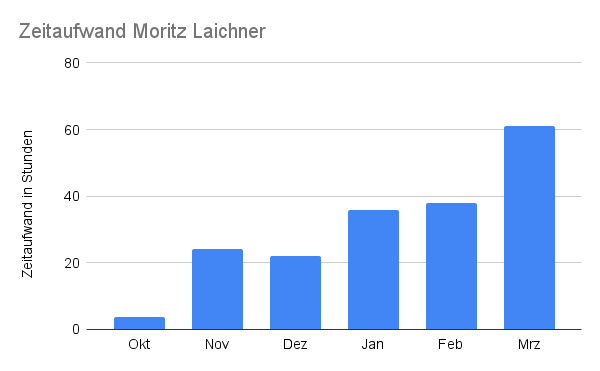
\includegraphics[width=.75\textwidth]{images/appendix/ZeitaufwandLaichner.png}
        \caption{Arbeitsstunden von Moritz Laichner verteilt auf die Monate}
    \end{center}
\end{figure}

\textbf{Verteilung der Arbeitszeit}
\begin{figure}[H]
    \begin{center}
        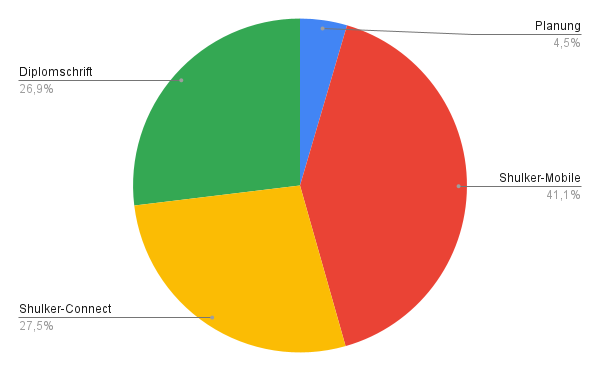
\includegraphics[width=.75\textwidth]{images/appendix/AufteilungLaichner.png}
        \caption{Verteilung der Arbeitszeit vom Moritz Laichner}
    \end{center}
\end{figure}